% !TeX root = ../thesis.tex

\chapter{Literature Survey}
\label{chap:literature_survey}

In this chapter, we will provide the background knowledge of the topic that was presented in Chapter 1. We will begin with an overview of the historical milestones of ECG and then move on to understand the basic knowledge of the cardiac cycle and the generation of ECG. We will then focus on understanding various ECG acquisition methods, emphasizing the advancement from multi-lead to single-lead technology. Next, we will explore the key challenges, such as noise interference, and discuss how edge computing and artificial intelligence have started to transform ECG monitoring, enhancing both performance and security. Finally, we will focus on the integration of edge computing on microcontrollers and explore different microcontrollers that can perform edge computing in terms of energy and operation. This review sets the stage for subsequent chapters highlighting challenges and emerging solutions in this field.

\section{Basic Knowledge of ECG}
\vspace{1em}
\subsection{Historical Development of ECG Technology}
\vspace{1em}
The study of phenomena such as the electric discharge of cramp fish and thunderstorms has been documented for many centuries. In 1781, Luigi Galvani made a groundbreaking discovery during a frog dissection. He observed that electrical stimulation of frog nerves resulted in muscle contraction, a phenomenon he termed "animal electricity." This discovery laid the biological foundations of electrophysiology for the first time~\cite{yang2015}.\\


\noindent Galvani's findings captured the attention of the scientific community. However, it was not until 1856 that Köllicker and Müller observed that the heart muscle itself could generate electrical activity. This observation was furthered nearly a decade later when, between 1869 and 1870, Alexander Muirhead recorded the first electrocardiogram (ECG) in London using a siphon instrument. Subsequently, in 1887, Augustus Waller used a capillary electrometer to record the heart's electrical activity~\cite{johansson2001}.\\

\noindent The significant advancement in ECG technology came from Dutch physiologist Willem Einthoven, who is often hailed as the father of electrocardiography. In 1893, Einthoven introduced the term "electrocardiography" into medical terminology. His major breakthrough occurred in 1901 with the invention of the string galvanometer, which revolutionized the recording of ECGs, as depicted in figure \ref{fig:einthoven_machine} . Furthermore, Einthoven simplified the electrode setup from the initially proposed five electrodes to just three. These electrodes were used to form the three standard leads, which facilitated the creation of Einthoven's triangle. This concept remains a fundamental part of ECG measurements today. Einthoven's dedication to advancing electrocardiography continued for over 25 years, culminating in him being awarded the Nobel Prize in 1924 for his contributions to medical science~\cite{alghatrif2012}~\cite{yang2015}

\begin{figure}[tb]
	\centering
	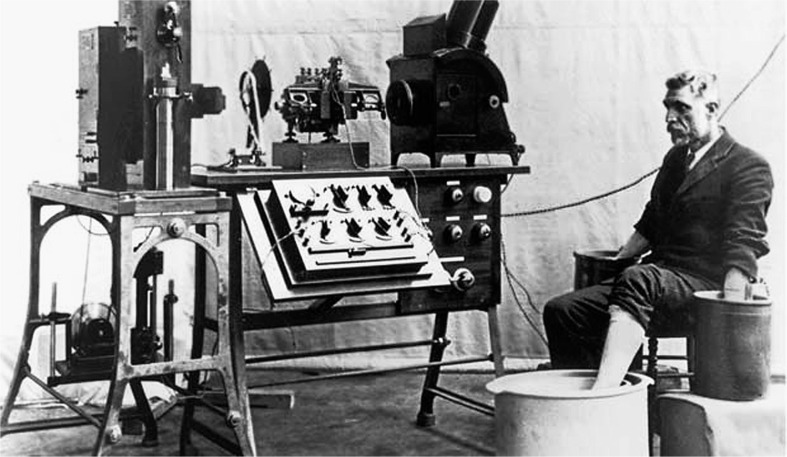
\includegraphics[width=0.8\textwidth]{images/einthoven_machine}
	\caption{Old string galvanometer electrocardiography~\cite{alghatrif2012}}
	\label{fig:einthoven_machine}
\end{figure}

\vspace{1em}

\noindent Despite numerous advancements and refinements in recording electrical potentials from the body's surface since Einthoven's string galvanometer, the fundamental principles of electrocardiography have remained largely unchanged.
\vspace{1em}


\subsection{Understanding the Cardiac Cycle}
\vspace{1em}
\noindent The heart comprises four chambers: the right and left atria, and the right and left ventricles. It also includes four valves: the tricuspid valve between the right atrium and ventricle, the mitral valve between the left atrium and ventricle, the pulmonary valve located between the right ventricle and the pulmonary artery, and the aortic valve situated in the outflow tract of the left ventricle, which controls blood flow to the aorta \cite{malminen1995} (as shown in Figure \ref{fig:heart_anatomy}).\\

\begin{figure}[tb]
	\centering
	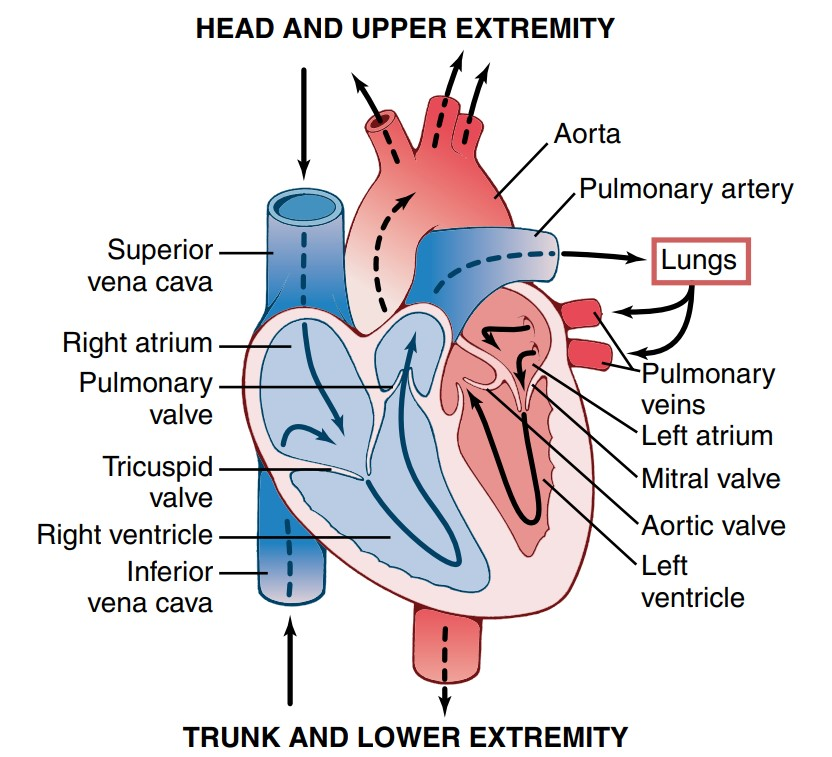
\includegraphics[width=0.8\textwidth]{images/anatomy of heart}
	\caption{Anatomy of the Heart~\cite{hall2015}}
	\label{fig:heart_anatomy}
\end{figure}


\noindent The cardiac cycle encompasses the events occurring from the beginning of one heartbeat to the beginning of the next. Blood distribution throughout the body is facilitated by the circulatory system, which includes two primary circuits: the pulmonary and the systemic circuits. The pulmonary circuit transports oxygen-deficient blood from the heart to the lungs and returns oxygenated blood to the heart, while the systemic circuit sends CO\textsubscript{2}-rich blood from the body to the heart and circulates oxygen-rich blood back to the body.\\

\noindent The cycle initiates on the right side of the heart, where deoxygenated blood enters the right atrium via the superior and inferior vena cavae. Upon contraction of the right atrium, blood flows through the tricuspid valve into the right ventricle. Once the right ventricle is filled, the tricuspid valve closes to prevent backflow into the atrium. The right ventricle then contracts, opening the pulmonary valve and pumping blood into the pulmonary artery to the lungs for oxygenation. After the blood is oxygenated in the lungs, it returns to the left atrium via the pulmonary veins.\\

\noindent Oxygenated blood is then drawn into the left ventricle through the mitral valve as the left atrium contracts. When the left ventricle is filled, the mitral valve closes to prevent backflow. Subsequent contraction of the left ventricle opens the aortic valve, allowing blood to be pumped into the aorta and distributed throughout the body. Following this, the aortic valve closes to prevent backflow to the left ventricle, which then relaxes in preparation for the next cycle of blood intake. This process constitutes one complete cardiac cycle \cite{hall2015, malminen1995}.


\subsection{Principles of ECG Signal Generation}
\vspace{1em}
\noindent A cardiac cycle is divided into two phases: diastole, a period of relaxation during which the heart fills with blood, and systole, a period of contraction. Diastole, also known as the re-polarization phase, involves the restoration of the cell's resting potential primarily through the efflux of potassium ions. Conversely, systole, or the depolarization phase, occurs when the cell becomes less negative relative to its resting state due to the influx of sodium ions through ion channels \cite{hall2015}.\\

\noindent The electrical activity in the heart originates from the sinoatrial (SA) node, located at the junction of the superior vena cava and the right atrium. Cells within the SA node are self-excitatory, often referred to as pacemaker cells, and typically initiate heartbeats at a rate of approximately 70 beats per minute. From the SA node, the electrical impulse spreads throughout the atria, causing atrial systole or depolarization. This impulse cannot directly reach the ventricles due to a fibrous septum that acts as an electrical insulator between the atria and ventricles. Thus, the transmission of the impulse from the atria to the ventricles is mediated by the atrioventricular node (AV node) through inter-nodal pathways. The AV node slows down the impulse, ensuring that atrial contraction completes before ventricular contraction begins, preventing simultaneous contraction of both chambers.\\

\noindent Following the AV node, the impulse travels through the bundle of His, which divides into left and right branches serving each ventricle. This conduction pathway extends into the Purkinje fibers, which distribute the impulse to the ventricular endocardial walls. As the electrical activity spreads from the inner to the outer walls of the ventricles, it triggers ventricular systole. Once all regions of the ventricular muscle have depolarized, they subsequently re-polarize.

\begin{figure}[h]
	\centering
	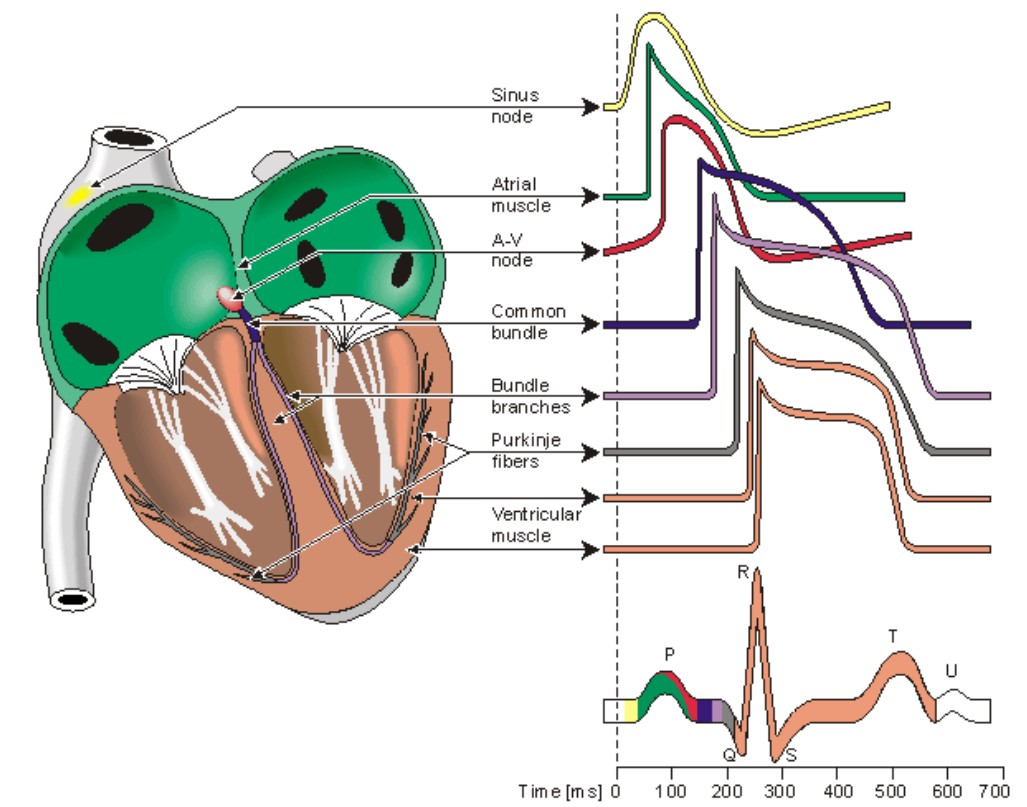
\includegraphics[width=0.8\textwidth]{images/action potention propagation of the heart}
	\caption{Waveform generated by the propagation of electrical signals through various specialized cardiac tissues, from the SA node to the ventricles~\cite{malminen1995}}
	\label{fig:ecg_signal}
\end{figure}

\noindent The ECG signal observed is essentially a superposition of action potentials from each cardiac tissue, demonstrating that the ECG is a composite of signals across different frequencies \cite{malminen1995}. This composite nature of the ECG signal helps in diagnosing various cardiac abnormalities by analyzing the waveform patterns.\\

\subsection{ECG Waveform}
\vspace{1em}
\noindent The resultant ECG signal consists of three principal waveforms:

\begin{itemize}
	\item \textbf{P wave:} This waveform results from the action potentials generated during the depolarization of the atria, which occurs just before atrial contraction begins.
	\item \textbf{QRS complex:} Comprising three individual waves—Q, R, and S—this complex is produced by the potentials generated during ventricular depolarization, just before the ventricles contract. Both the P wave and the QRS complex represent depolarization waves.
	\item \textbf{T wave:} Known as the repolarization wave, the T wave is generated as the ventricles recover from the state of depolarization.
\end{itemize}

\begin{figure}[h]
	\centering
	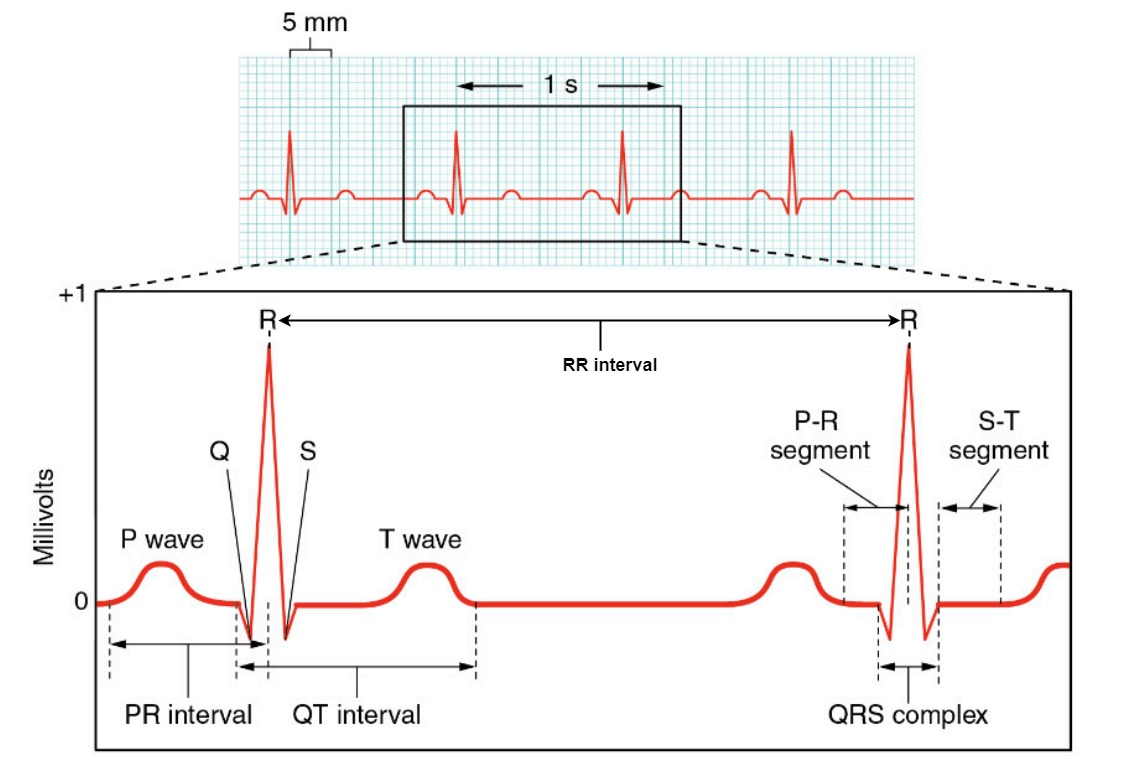
\includegraphics[width=0.8\textwidth]{images/temp}
	\caption{Illustrates a normal ECG signal, highlighting various intervals and signal markings that are crucial for understanding the heart's morphology~\cite{mamun2022}.}
	\label{fig:normal_ecg}
\end{figure}

\noindent The table \ref{tab:ecg_waves} below specifies the typical frequency and amplitude values for each type of ECG waveform:

\begin{table}[h]
	\centering
	\caption{Characteristics of ECG Waves\cite{zyout2023}}
	\begin{tabular}{|l|l|l|}
		\hline
		\textbf{ECG Wave} & \textbf{Amplitude} & \textbf{Frequency} \\ \hline
		P wave & 0.25 mV & 5-30 Hz \\ \hline
		QRS complex & 1.6 mV (R peak) & 8-50 Hz \\ \hline
		T wave & 0.1-0.5 mV & 0-10 Hz \\ \hline
	\end{tabular}
	\label{tab:ecg_waves}
\end{table}

\noindent In this thesis, the detection of atrial fibrillation—specifically through heart rate variability—is centered on identifying R peaks within the frequency range of 8-50 Hz, with peak power occurring in the range of 4 to 12 Hz \cite{murthy1978}.\\

\section{ECG Acquisition Techniques}
\vspace{1em}
\noindent Electrical activities of the heart can be detected on the skin using electrodes. An ECG machine captures these activities and graphically displays them, showing the heart's electrical potential or voltage as it fluctuates throughout a cardiac cycle.\\

\subsection{Three-Lead ECG Systems}\label{einthoven}
\vspace{1em}
\noindent The three-lead ECG system operates based on the principles first introduced by Willem Einthoven, who developed the concept of the three bipolar limb leads (I, II, and III). These leads form what is known as Einthoven's Triangle, a fundamental setup in the field of electrocardiography, as illustrated in Figure~\ref{fig:einthoven_triangle}.

\begin{figure}[h]
	\centering
	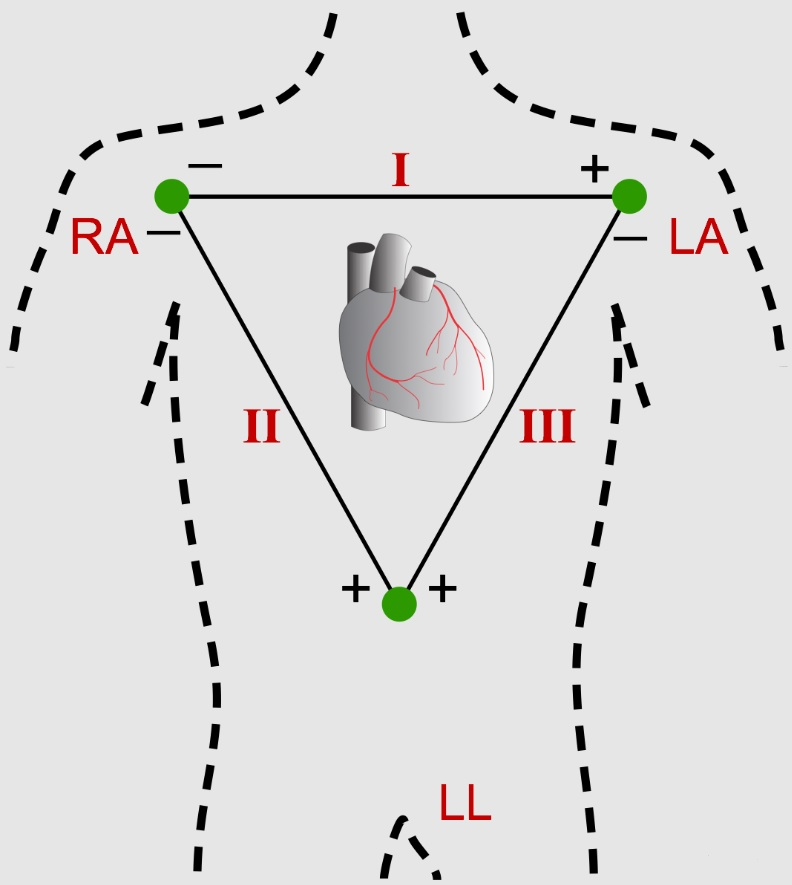
\includegraphics[width=0.5\textwidth]{images/einthoven traingle}
	\caption{Einthoven's Triangle~\cite{cvphysiology}}
	\label{fig:einthoven_triangle}
\end{figure}

\noindent This setup involves placing electrodes on the left arm (LA), right arm (RA), and left leg (LL). The potential difference measured across each lead is derived from the relative placement of these electrodes according to the Einthoven Triangle:\\
\begin{itemize}
	\item \textbf{Lead I:} Measures the potential difference between the left arm (LA) and right arm (RA).
	\item \textbf{Lead II:} Measures the potential difference between the left leg (LL) and right arm (RA).
	\item \textbf{Lead III:} Measures the potential difference between the left leg (LL) and left arm (LA).
\end{itemize}

\noindent Three-lead ECG systems are commonly utilized in Mobile Cardiac Telemetry (MCT) for continuous monitoring, especially useful for detecting cardiac artifacts\cite[chap. 1, p. 4]{conover2002}\cite{tsang2013}.\\

\subsection{12-Lead ECG Systems}
\vspace{1em}
\noindent Building on Einthoven's foundational work, Goldberger expanded the diagnostic capabilities of ECG by introducing augmented leads known as aVR, aVL, and aVF. These leads were designed to provide additional views of cardiac activity to address gaps in the data provided by the original three leads. Goldberger employed the "Wilson central terminal" (WCT), a reference point established by connecting the three limb electrodes (right arm, left arm, and left leg). The electric potentials for the augmented leads relative to the WCT are specified the below equations-\cite{wagner2013, malminen1995}:

\begin{equation}
	aVF = LL - 0.5 \times (RA + LA)
\end{equation}
\begin{equation}
	aVL = LA - 0.5 \times (RA + LL)
\end{equation}
\begin{equation}
	aVR = RA - 0.5 \times (LA + LL)
\end{equation}

\noindent Figure~\ref{fig:leads} below illustrates the configurations of limb leads (I-III) and augmented leads (aVR, aVL, aVF), which together provide comprehensive information about the frontal plane of the heart.

\begin{figure}[H]
	\centering
	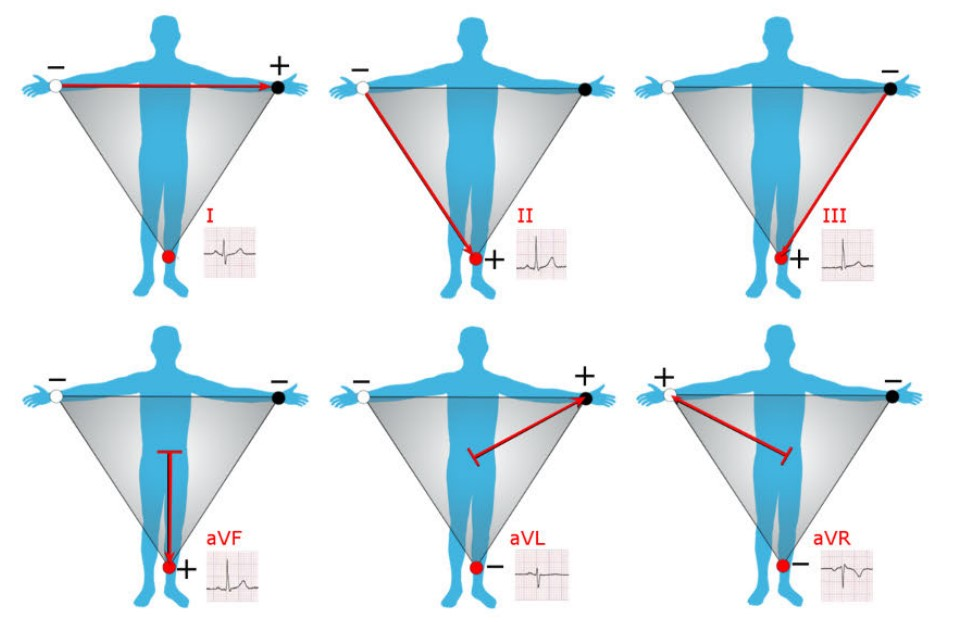
\includegraphics[width=0.7\textwidth]{images/3lead and augumented lead}
	\caption{Illustration of Limb Leads(Top) and Augmented Leads(Bottom) \cite{wasimuddin2020}}
	\label{fig:leads}
\end{figure}

\noindent To further enhance the understanding of the heart’s transverse plane, Wilson introduced six precordial leads (V1 to V6). In this setup, the positive electrode is connected to a specific precordial site, while the negative electrode is linked to the WCT\cite{hall2015, malminen1995}. The potential difference between these electrodes defines the voltage for each precordial lead given as-

\begin{equation}
	VL = V'L - \text{WCT}
\end{equation}

Here, \( V'L \) represents the voltage recorded at the L\textsuperscript{th} precordial electrode, and WCT is calculated as:

\begin{equation}
	\text{WCT} = \frac{1}{3} \times (RA + LA + LL)
\end{equation}

\noindent The combination of limb leads, augmented leads, and precordial leads comprises the 12-lead ECG system, which utilizes nine electrodes (three for the limbs and six for the precordial) to generate twelve distinct waveforms corresponding to each lead.Additionally, a Right lead electrode is used for reference as discussed in \ref{RLD}. This system is depicted in Figure \ref{fig:12_lead_ecg}.
\begin{figure}[H]
	\centering
	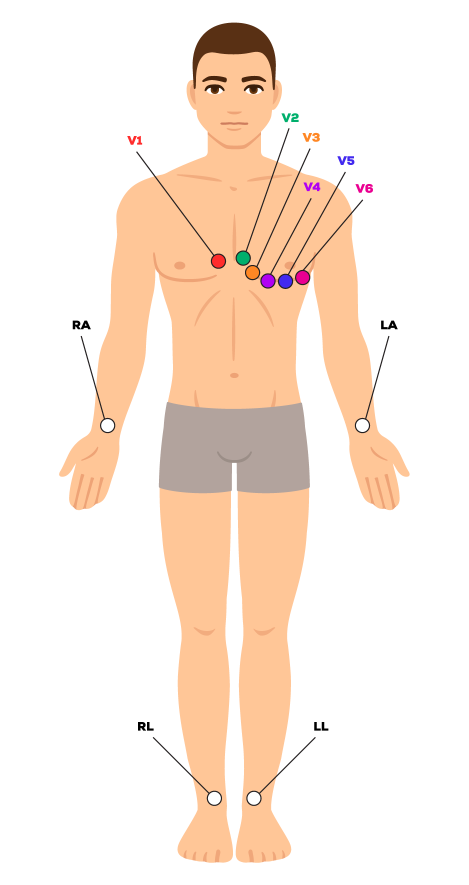
\includegraphics[width=0.3\textwidth]{images/12lead placement}
	\caption{12-Lead ECG Electrode Configuration \cite{cardiacdirect_ecg}}
	\label{fig:12_lead_ecg}
\end{figure}

\noindent The 12-lead ECG is considered the gold standard for monitoring all types of cardiac activities. Despite its comprehensive capabilities, the complex arrangement of electrodes makes the 12-lead ECG less suitable for daily, long-term monitoring. On the other hand, the three-lead system, with a specificity of 98.7\% for detecting atrial fibrillation (AF), is often preferred for this purpose due to its simpler setup and effectiveness in diagnosing AF \cite{kristensen2016}.

\subsection{Single-Lead ECG Systems}
\vspace{1em}
\noindent Single-lead ECG systems have gained increasing relevance in recent years. They utilize just one of the leads from the Einthoven triangle, making them particularly suited for prolonged continuous monitoring of ECG data, typically over 24 to 48 hours. Their simplicity and ease of use make them ideal for outpatient settings and home monitoring.\\

\noindent One significant challenge in single-lead ECG systems is the necessity for a specialized front-end ECG acquisition stage. This requirement stems from the absence of a reference electrode, which is usually provided by the driven right leg (DRL) circuit \ref{RLD}. The front-end design must compensate for this by ensuring a high Common Mode Rejection Ratio (CMRR) \cite{babusiak2015}. This design enhances the ability of the differential amplifier to discriminate between the desired biological signals and unwanted noise, thereby improving the quality and reliability of the ECG data captured.\\

\noindent In this thesis, we explore such a front-end circuit, focusing on its design and implementation within our ECG detection system. This examination will provide insights into the technical adaptations needed to optimize single-lead ECG systems for effective cardiac monitoring.\\


\section{Challenges in ECG Monitoring}
\vspace{1em}
\noindent Accurate diagnosis from ECG readings relies heavily on signal quality. The clinically useful information in an ECG waveform is typically found within the frequency range of 0.05 to 100 Hz and has a dynamic range of 1 to 10 mV \cite{Velayudhan2016NoiseAA}. High-quality signals are crucial for the accuracy and reliability of ECG diagnoses. However, various types of noise can interfere with signal acquisition, merging with the ECG signal and potentially hindering accurate diagnosis.\\

\noindent Noise in ECG signals generally falls into two categories: high-frequency and low-frequency noises. High-frequency noises like Electromyogram noise, Additive white noise, and power line Interference while Low-frequency noises include baseline wandering and motion artifacts \cite{Velayudhan2016NoiseAA}.\\

\subsection{Types of Noise in ECG Signals}\label{noises}
\vspace{1em}
\subsubsection{Power Line Interference}
\vspace{1em}
\noindent Power line interference is a type of common-mode noise affecting ECG signals due to electromagnetic fields generated by power lines. This interference typically manifests as a 50/60 Hz sinusoidal wave, often accompanied by harmonics, resulting from AC fields produced by looped wires, poor grounding, or bad contacts. Suppressing this interference is crucial as it can obscure the low-amplitude signals of the ECG, such as the P, Q, S, and T waves \cite{Velayudhan2016NoiseAA,Kher2019SignalPT}.

\begin{figure}[h]
	\centering
	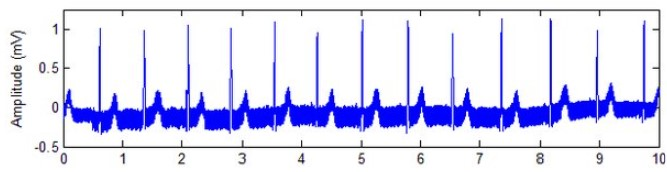
\includegraphics[width=0.8\textwidth]{images/powerline noise}
	\caption{Power Line Interference in ECG \cite{Maggio2012Quantification}}
	\label{fig:power_line_interference}
\end{figure}

\subsubsection{Baseline Wander}
\vspace{1em}
\noindent Baseline wander, or drift, occurs when the baseline of the ECG signal shifts vertically instead of remaining straight. This noise is predominantly caused by patient movement and respiration, typically at frequencies below 1 Hz \cite{Kher2019SignalPT}.

\begin{figure}[h]
	\centering
	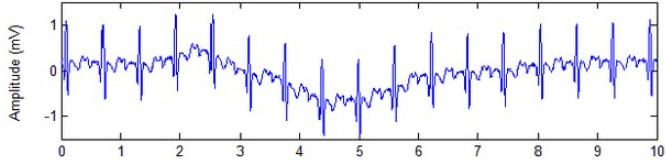
\includegraphics[width=0.8\textwidth]{images/baseline wander}
	\caption{Baseline Wander in ECG \cite{Maggio2012Quantification}}
	\label{fig:baseline_wander}
\end{figure}

\subsubsection{Electromyogram (EMG) Noise}
\vspace{1em}
\noindent Electromyogram noise is high-frequency interference arising from muscle activity during the recording of ECG, which can reach frequencies up to 10 kHz \cite{Velayudhan2016NoiseAA,Kher2019SignalPT}. This type of noise interferes with the ECG signal.

\begin{figure}[h]
	\centering
	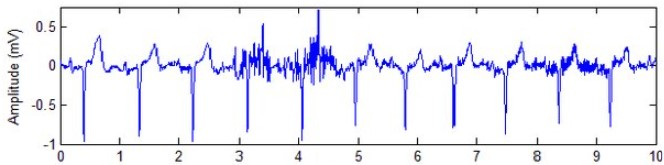
\includegraphics[width=0.8\textwidth]{images/emg_noise}
	\caption{EMG Noise in ECG \cite{Maggio2012Quantification}}
	\label{fig:emg_noise}
\end{figure}

\subsubsection{Motion Artifacts}
\vspace{1em}
\noindent Motion artifacts, similar to baseline wander, significantly affect ECG signals. They can distort the entire PQRST complex due to changes in skin impedance caused by skin stretching near the electrodes. These artifacts typically occur in the 1 to 10 Hz frequency range~\cite{Kher2019SignalPT} and can be seen in Figure \ref{fig:motion_artifacts}.

\begin{figure}[h]
	\centering
	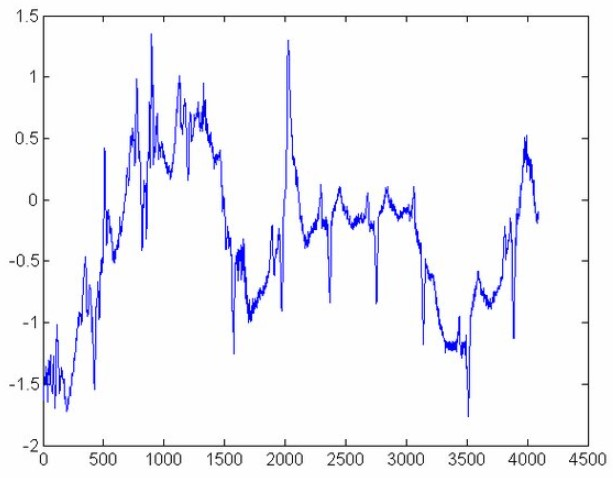
\includegraphics[width=0.6\textwidth]{images/motionArtifacts}
	\caption{Motion Artifacts in ECG \cite{Kher2019SignalPT}}
	\label{fig:motion_artifacts}
\end{figure}

\noindent Understanding and addressing these noise types is essential for improving ECG signal quality and ensuring accurate cardiac monitoring and diagnosis.\\


\subsection{Strategies for Noise Reduction}
\vspace{1em}
\noindent Reducing noise in ECG signals involves distinguishing and removing unwanted interference while preserving the original signal's integrity. Effective noise reduction can be achieved primarily through two methods: utilizing a front-end circuit to diminish common mode noise before it reaches the differential stage, and employing various filtering techniques to isolate the essential frequency components of the ECG signal. We will explore a notable method for common mode noise reduction and some filtering techniques commonly referenced in literature.\\

\subsubsection{Driven Right Leg (RLD)}\label{RLD}
\vspace{1em}
\noindent The RLD technique enhances ECG systems by mitigating common mode noise using an additional electrode attached to the right leg. This electrode, while not directly involved in diagnostic measurements, serves as a reference point for the ECG system and redirects common mode noise back to the body. Originally introduced by Winter and Webster, the RLD method typically employs a differential amplifier as a front-end circuit to further reduce common mode noise and enhance signal sensitivity \cite{Winter1983Driven}.\\

\noindent The RLD utilizes the "Wilson central terminal technique," where a node averaging all electrode potentials is created. This node effectively nullifies differential mode signals and provides a low-resistance pathway for common mode signals. As illustrated in Figure \ref{fig:rld_circuit}, common mode signals ($I_3$), facilitated by averaging resistors ($R_a$), are inverted and re-introduced to the body through the right leg electrode $RL$, enhancing overall ECG signal clarity.

\begin{figure}[htbp]
	\centering
	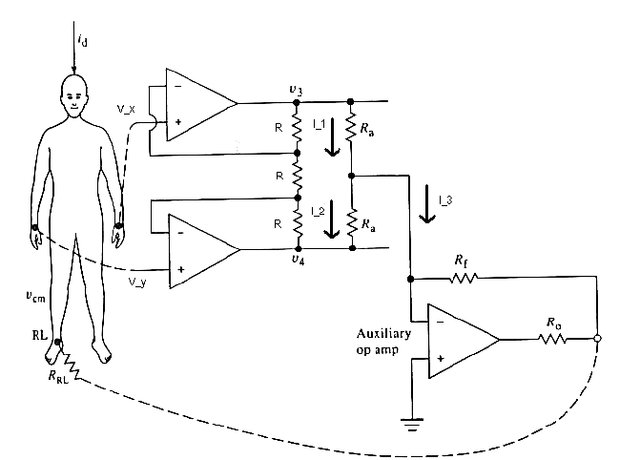
\includegraphics[width=0.7\textwidth]{images/driven right leg}
	\caption{Driven Right Leg Circuit Schematic \cite{Saha2018Design}}
	\label{fig:rld_circuit}
\end{figure}

\subsubsection{Filtering Techniques}
\vspace{1em}
\noindent Various filtering techniques are discussed extensively in the literature to address different types of noise \cite{Luo2010Review}. Filtering techniques are normally classified into two types: digital filtering, which is done at the backend after extracting the raw noisy data, and analog filtering, which is done during the extraction of the ECG signal.

\begin{itemize}
	\item \textbf{Notch Filters:} These are used specifically to eliminate power line interference, typically at 50/60 Hz.
	\item \textbf{Low-Pass Filters:} These filters remove high-frequency noise above 150 Hz, which is beyond the range of typical ECG signals.
	\item \textbf{High-Pass Filters:} Employed to eliminate low-frequency noises such as baseline drift and motion artifacts.
	\item \textbf{Antialiasing Filters:} These are crucial just before the analog-to-digital conversion process, particularly when the sampling frequency does not meet the Nyquist criterion. This helps prevent aliasing from corrupting the digital ECG signal.
\end{itemize}

\noindent The selection of a specific filter depends on the characteristics of the ECG signal needed for accurate diagnosis and the type of noise interference present in the signal environment.\\

\section{Architectures for ECG Data Acquisition}
\vspace{1em}
\noindent Wearable health devices are increasingly favored for their ability to monitor heart activity continuously, minimize discomfort, and interfere with daily activities. These devices, typically battery-powered, support both real-time and offline data monitoring. Understanding the architecture of these systems, as well as identifying areas for improvement, is crucial for advancing their effectiveness.

\subsection{Remote and Offline Monitoring Architectures}
\vspace{1em}
\noindent According to various literature reviews, the architecture depicted in Figure \ref{fig:wbna_architecture} represents a generic setup for wearable continuous monitoring utilized in both researched prototypes and commercial products. This system architecture is often referred to as a “Wireless Body Area Network” (WBAN).

\begin{figure}[htbp]
	\centering
	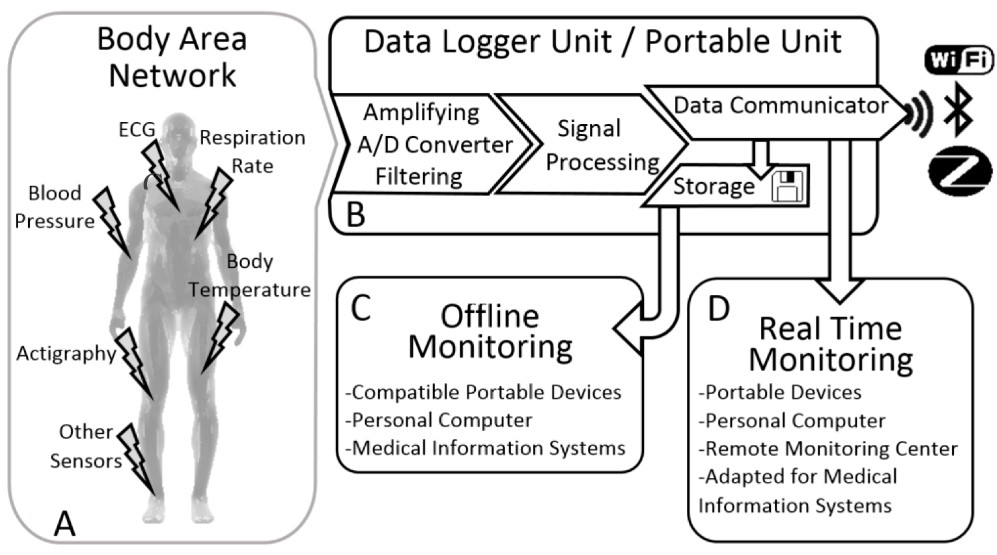
\includegraphics[width=0.7\textwidth]{images/remote architecture}
	\caption{WBAN Architecture~\cite{Dias2018Wearable}}
	\label{fig:wbna_architecture}
\end{figure}

\noindent\textbf{Body Area Network (BAN)}

\noindent A BAN consists of interconnected sensor nodes, each dedicated to monitoring specific body parameters. Each node is equipped with a sensor system, a controller, and a memory unit. Data, whether raw or filtered, is transmitted from the sensor nodes to a central data logger unit for further processing. Connection to a central portable unit via wired or wireless means centralizes and synchronizes the data, crucial for effective continuous monitoring. In the case of continuous monitoring, only a single node is connected directly to the Data logger unit for processing, storing, and transmitting \cite{Dias2018Wearable, Pantelopoulos2010Survey}.\\

\noindent\textbf{Data Logger/Portable Unit}

\noindent This component logs data from various sensor nodes. It receives analog signals, converts them to digital via an A/D converter, and processes the data to extract additional information, such as heart rate from ECG, using measurements like RR peak distances. Data can be utilized for immediate real-time monitoring or stored for later analysis \cite{Dias2018Wearable}.\\

\noindent\textbf{Real-Time Monitoring}

\noindent Advancements in AI allow data from the portable unit to be sent to remote servers where various machine learning algorithms classify different abnormalities in real time. Transmission utilizes wireless protocols such as Bluetooth, BLE, Zigbee, GSM, and WiFi \cite{Dias2018Wearable, Shaown2019IoT}.\\

\noindent\textbf{Offline Monitoring}

\noindent Data can also be archived on portable storage devices such as micro SD cards or USB drives for future analysis by medical professionals or for personal health records \cite{Dias2018Wearable}.\\

\noindent\textbf{Challenges}

\noindent Despite the benefits, several challenges persist in this architecture as\cite{Muhoza2023Power, Lim2010Security}-:

\begin{itemize}
	\item \textbf{Power Consumption:} Continuous data transmission, especially using WiFi or BLE, can be energy-intensive.
	\item \textbf{Latency:} High data traffic can lead to congestion and increased latency.
	\item \textbf{Security:} Ensuring data privacy and security remains a concern. Encrypting data before transmission requires considerable computational power, which may not be feasible for battery-operated devices.
\end{itemize}


\subsection{Edge-Based Monitoring Architectures Using AI}
\vspace{1em}
\subsubsection{Edge AI-related Work}

\noindent Edge AI involves integrating artificial intelligence algorithms directly into microcontroller-based devices, contrasting with remote AI, which relies on cloud or remote servers for computation. Research indicates that Edge AI significantly reduces energy consumption and latency compared to cloud-based AI solutions \cite{Muhoza2023, Himeur2024, Vita2020}. A notable study \cite{Muhoza2023} employed an ARM Cortex-based microcontroller to run a DCNN model that predicted human activity from accelerometer data, highlighting the efficiency of Edge AI through two scenarios:\\

\noindent\textbf{Scenario 1 (Remote AI):}

\noindent In this scenario, as soon as the data is acquired from the accelerometer sensor, it is directly transmitted to a remote server using BLE communication for AI computation as shown in Figure \ref{fig:remote_ai}. In this scenario, there is no intervention of the AI algorithm used at the sensor node \cite{Muhoza2023}.

\begin{figure}[h]
	\centering
	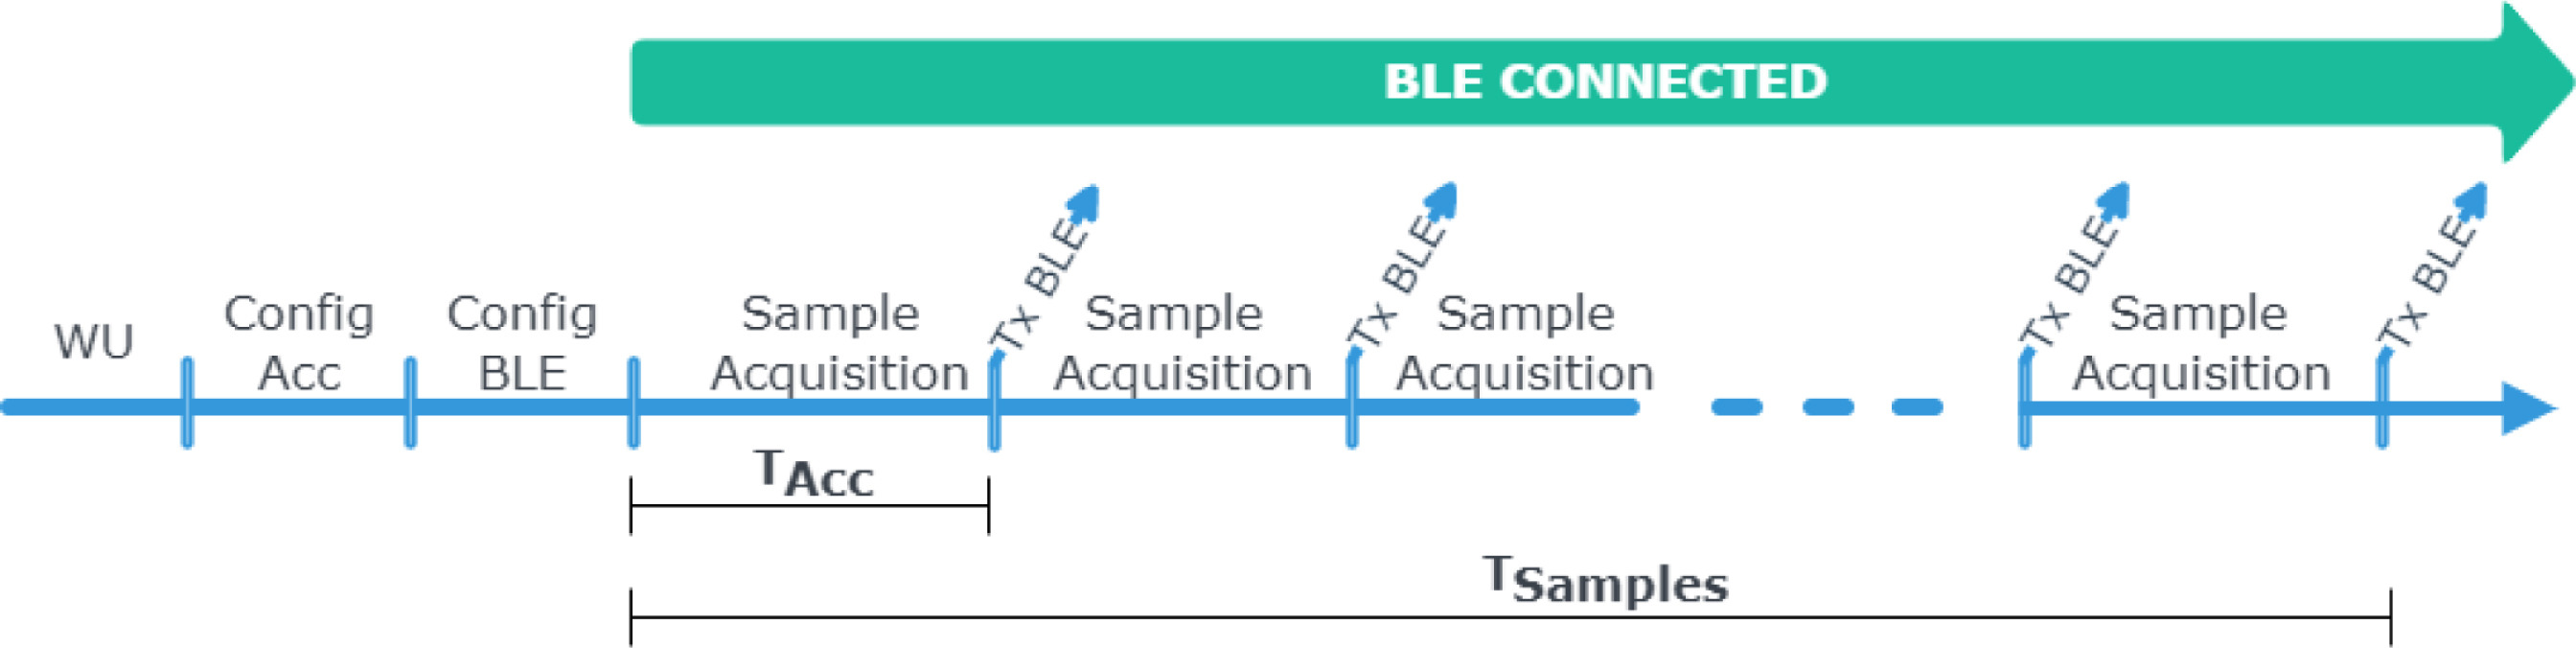
\includegraphics[width=0.8\textwidth]{images/senerio1}
	\caption{Remote AI Data Flow~\cite{Muhoza2023}}
	\label{fig:remote_ai}
\end{figure}

\noindent\textbf{Scenario 2 (Edge AI):}

\noindent In this scenario, the DCNN model running on an edge microcontroller processes data locally every 100 samples. It achieves an F1 score of 98.3\% in classifying human activities. DCNN results classification is buffered locally and only transmitted when the buffer is full, significantly reducing BLE usage and power consumption, as BLE is only active and connected when the buffer is ready to transmit. The DCNN model used consisted of two successive 1D convolution layers, a pooling layer, two fully connected layers, and a softmax layer for activity prediction \cite{Muhoza2023}.

\begin{figure}[h]
	\centering
	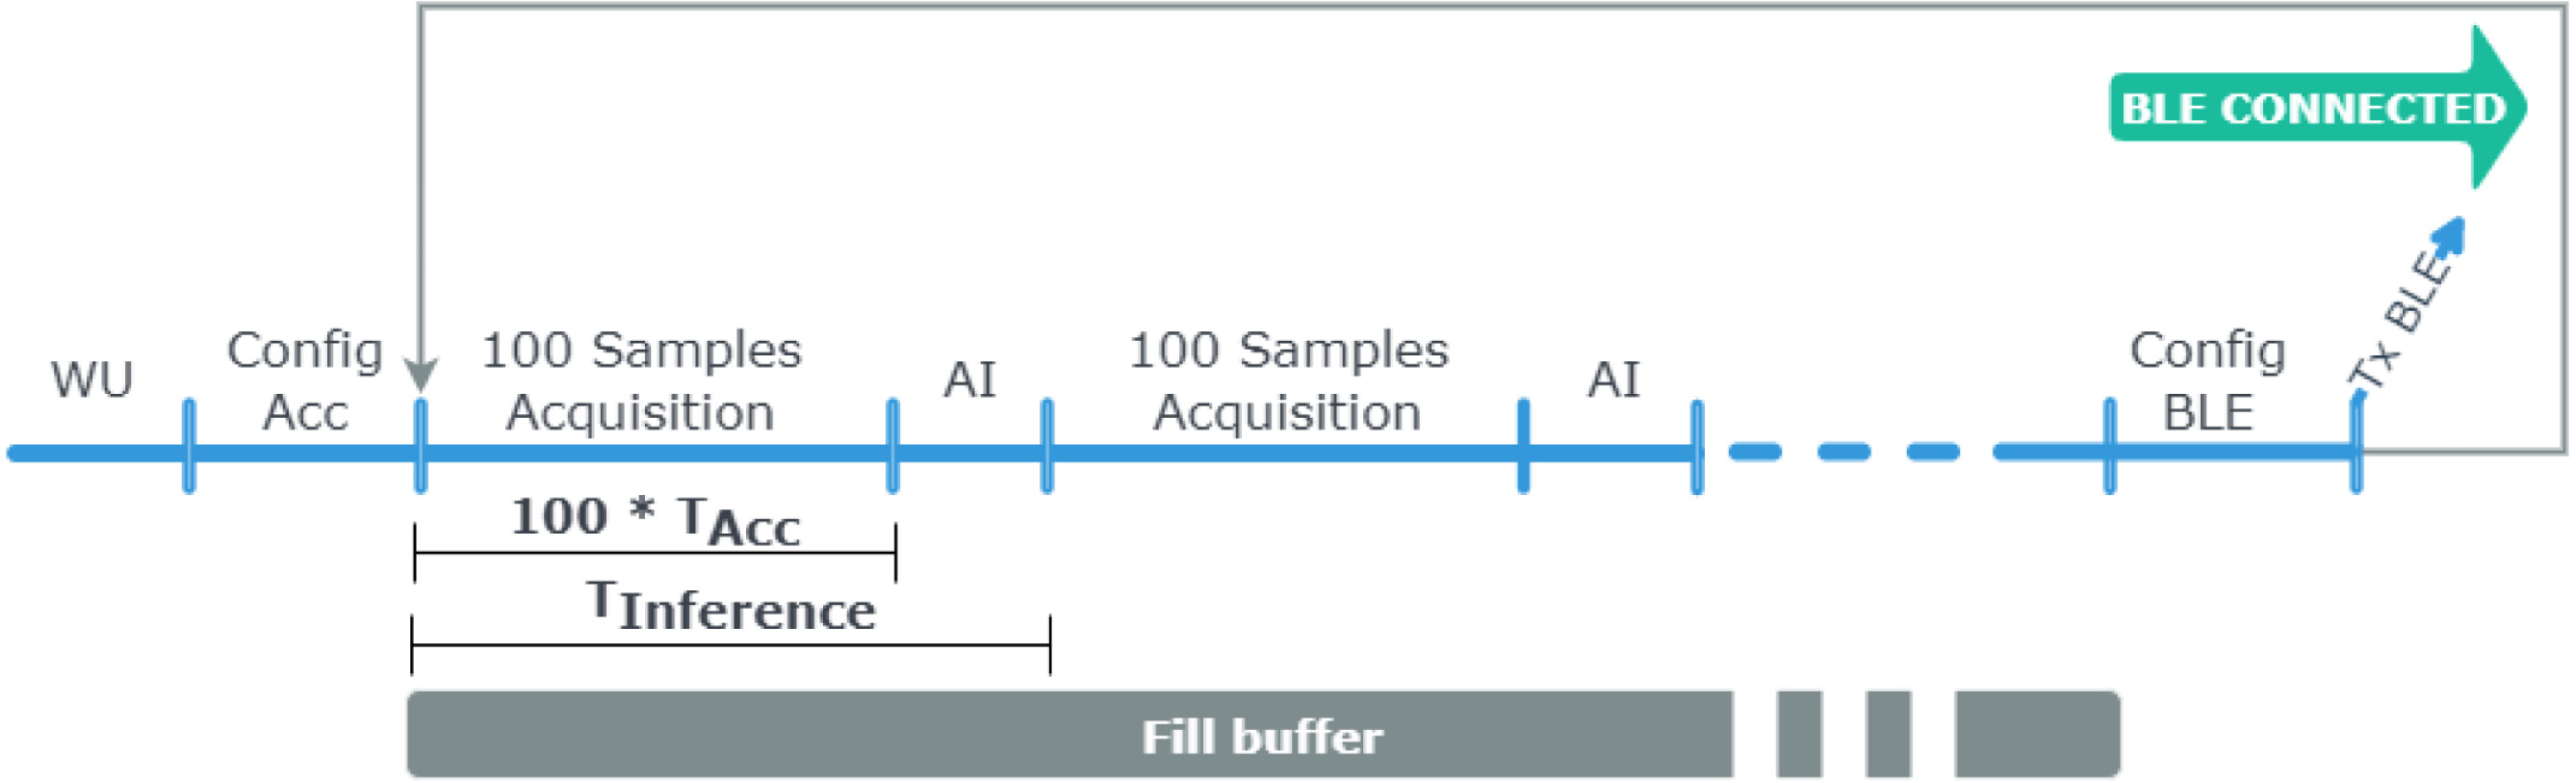
\includegraphics[width=0.8\textwidth]{images/SENERIO2}
	\caption{Edge AI Data Flow~\cite{Muhoza2023}}
	\label{fig:edge_ai}
\end{figure}

\noindent Comparative analysis showed that Scenario 2 saved up to 20\% battery life over an hour compared to Scenario 1, while also minimizing Bluetooth congestion, which is notable since the BLE module consumes considerable power during data transmission \cite{Muhoza2023}.

\begin{figure}[h]
	\centering
	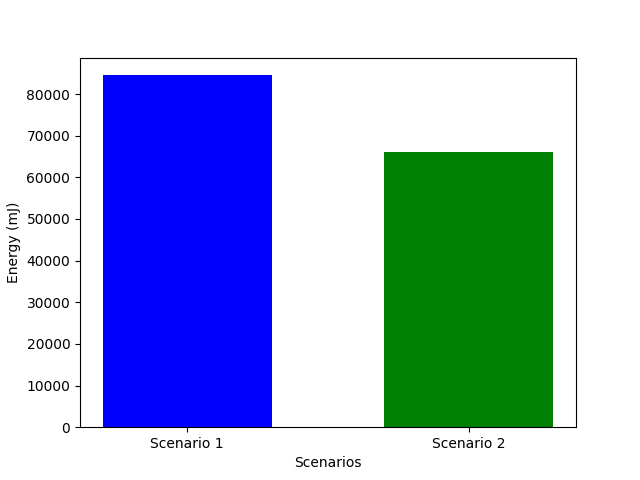
\includegraphics[width=0.7\textwidth]{images/senerio comparision}
	\caption{Battery Usage Comparison (redrawn from \cite{Muhoza2023})}
	\label{fig:battery_usage}
\end{figure}

\subsubsection{Edge AI-based Architecture}
\vspace{1em}
\noindent A survey of literature on Edge AI underscores the need for integrating AI processing within wearable monitoring systems to enhance remote monitoring architectures. By incorporating an Edge AI element just before data transmission to a remote server, a new architecture emerges, significantly optimizing power and data latency \cite{Muhoza2023, Shaik2023, Mujawar2020, Ashfaq2022}. This architecture utilizes DNN models to process digital data post-A/D conversion, dramatically enhancing battery efficiency and reducing latency.

\begin{figure}[h]
	\centering
	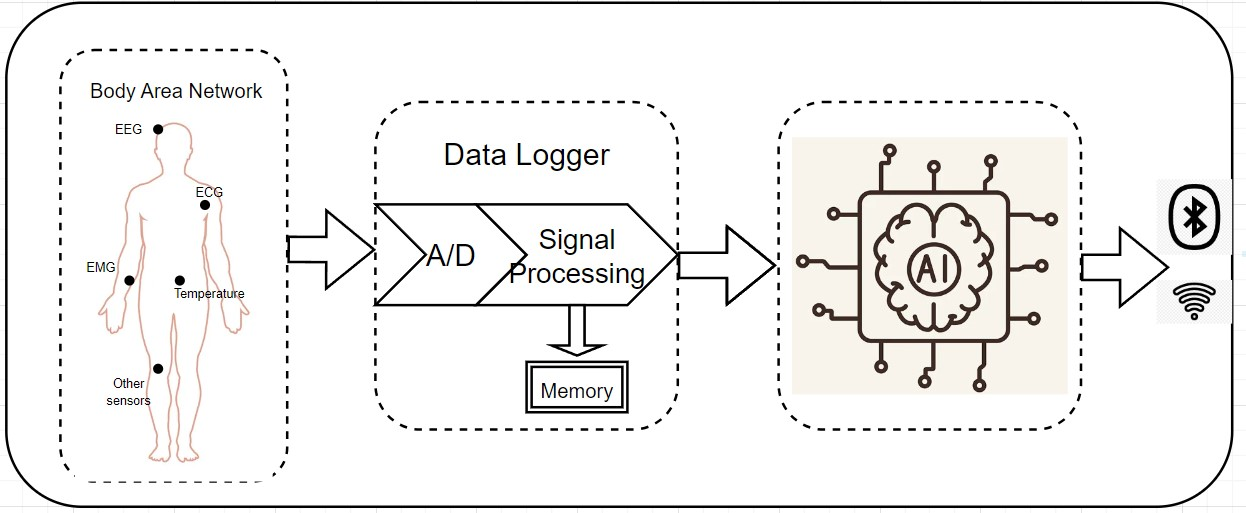
\includegraphics[width=0.8\textwidth]{images/ai on edge arch}
	\caption{Edge AI-Based Architecture (redrawn from \cite{Muhoza2023, Shaik2023, Mujawar2020, Ashfaq2022})}
	\label{fig:edge_ai_based_architecture}
\end{figure}

\noindent This thesis will explore this Edge AI-based architecture, comparing its performance with traditional remote and offline monitoring setups in terms of energy efficiency and effectiveness in detecting atrial fibrillation (AF) in ECG signals.\\

\subsubsection{Edge AI-based DNN Accelerators}
\vspace{1em}
\noindent Recent advancements in deep neural networks (DNN) have led to models that more closely mimic real-world sensory systems, though they have become computationally and memory-intensive. Deploying such models on microcontrollers often results in systems that are unsuitable for battery-powered devices due to high energy demands.\\

\noindent To mitigate energy and memory inefficiency, novel hardware architectures have been developed specifically for handling DNN-based workloads \cite{Moss2023, Reuther2021}. These architectures typically feature on-chip memory to minimize power consumption and latency associated with data transfer from off-chip memory. They also include large computational arrays for performing operations such as addition and matrix multiplication, and dedicated data flow paths between computational cores to enhance data reuse. Most operate with low-precision computing, like 8-bit operations, to balance performance with energy efficiency. Figure \ref{fig:dnn_hardware_comparison} illustrates a comparison of power usage against GOPs (Giga Operations per second) for various hardware architectures designed by different companies \cite{Moss2023}.\\

\begin{figure}[h]
	\centering
	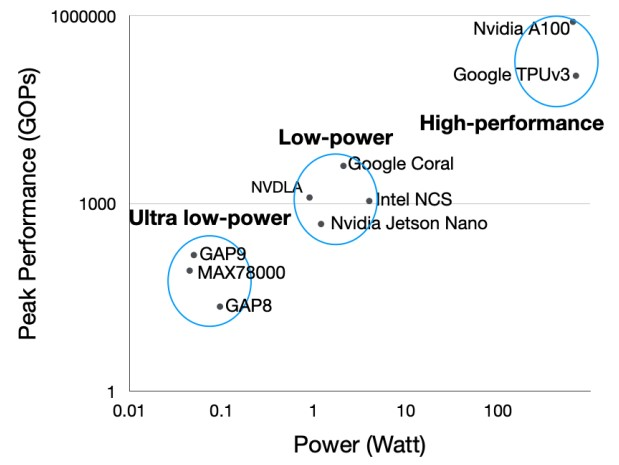
\includegraphics[width=0.6\textwidth]{images/power vs gops}
	\caption{Comparison of Power Consumption and Computational Capacity in DNN Hardware Architectures~\cite{Moss2023}}
	\label{fig:dnn_hardware_comparison}
\end{figure}

\noindent Among these, ultra-low power hardware accelerators are particularly suited for battery-operated biosensing devices. The Max78000, for example, is a system-on-chip that executes neural networks with ultra-low power consumption. It combines a dual-core microcontroller (ARM Cortex-M4 and a RISC-V co-processor) with a dedicated CNN hardware accelerator, capable of supporting deep CNN networks up to 64 layers with 64 parallel processors. This allows for both 1D and 2D convolution processing. The CNN engine includes its own weight memory of 441KB and supports up to 8-bit weight precision \cite{MAX78000-datasheet}. Figure \ref{fig:max78000_hardware} shows the hardware architecture of the Max78000.

\begin{figure}[h]
	\centering
	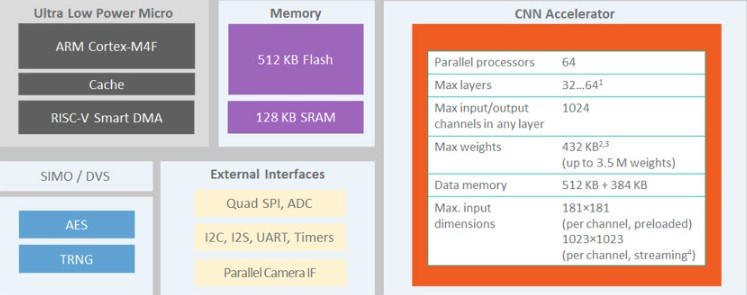
\includegraphics[width=0.8\textwidth]{images/max78000arch}
	\caption{MAX78000 Hardware Architecture~\cite{analog-devices-max78000-app-note}}
	\label{fig:max78000_hardware}
\end{figure}

\noindent This thesis will explore the integration of the MAX78000-based feather board with an ECG circuit board to classify heart rate abnormalities and related diseases.\\

\section{Security in Medical Sensing}
\vspace{1em}
\noindent As medical sensing devices increasingly integrate with the Internet of Things (IoT), securing sensitive health data becomes paramount. These devices frequently transmit data to remote servers for analysis and storage, making them potential targets for cybersecurity threats. Breaches can compromise patient privacy and lead to serious health risks, such as incorrect diagnoses or inappropriate medical interventions \cite{Paul2023, Abdunabi2023}.

\begin{itemize}
	\item \textbf{Vulnerability of Medical Data:} The integration of IoT in medical devices exposes them to various security vulnerabilities, particularly at the point of data transmission. Devices using wireless communication technologies like Bluetooth Low Energy (BLE) or Zigbee are especially susceptible to eavesdropping and interference \cite{Paul2023, Bresson2004}. The potential for data interception or manipulation can lead to catastrophic outcomes, including the administration of incorrect medical treatments.

	\item \textbf{Strategies for Enhancing Security:} Literature on the topic suggests multiple approaches to protect against these vulnerabilities. The implementation of strong encryption protocols is a primary method for securing data transmitted between IoT devices and remote servers. Encrypting data ensures that even if data interception occurs, the information remains unintelligible without the proper decryption keys \cite{Paul2023, Bresson2004}.

	\item \textbf{Security Implementation Challenges:} Encryption enhances data security but also adds extra computational overhead and power consumption. Implementing a security node just before sending data to the server involves substantial energy-intensive operations.

	\item \textbf{Edge AI for Enhanced Security:} Utilizing edge AI architecture can significantly reduce the amount of data needing transmission by processing data directly on the device. This approach limits the exposure of raw data to potential security threats. For instance, devices can analyze and process ECG data locally to determine the presence of atrial fibrillation and only transmit the essential summarized data or alerts to healthcare providers. This reduces the bandwidth needed for data transmission, decreases the risk of data interception, and conserves energy \cite{Paul2023}.
\end{itemize}

\noindent This thesis explores the use of the Infineon OPTIGA™ Trust M, a security solution integrated into the edge AI architecture. This module provides robust security by handling cryptographic operations directly on the chip, thus safeguarding data integrity and authenticity from the point of capture to storage and analysis. The integration of such security elements demonstrates how advanced hardware can be leveraged to enhance data protection in medical IoT devices without excessive power consumption \cite{infineon-optiga-trust}.\\
